\documentclass{beamer}
\usetheme{Boadilla}
\usepackage{graphicx}
\usepackage{multicol}
\graphicspath{ {./images} }

\title {Atividade 3 IHC}
\subtitle {Exemplos relacionados à acessibilidade digital}
\author {Henrique Tsuyoshi Yara N° 11796083}
\institute {USP - Universidade de São Paulo}

\begin{document}

\begin{frame}{\titlepage}
\end{frame}

\begin{frame}{Índice}
\begin{multicols}{2}
  \tableofcontents
\end{multicols}
\end{frame}

\section{Princípio Perceptível}
\subsection{1.1 - Conteúdo não textual}

\begin{frame}{Conteúdo não textual - Exemplo Ruim}

Princípio: Princípio Perceptível

WCAG: 1.1 - Conteúdo não textual

\begin{itemize}
	\item Podemos ver no site do mourao restaurante que as imagens ou não possuem o atributo \textbf{alt} ou possuem um \textbf{alt} que não condiz com a imagem, no exemplo abaixo vemos:
\end{itemize}
\begin{figure}
    \centering
    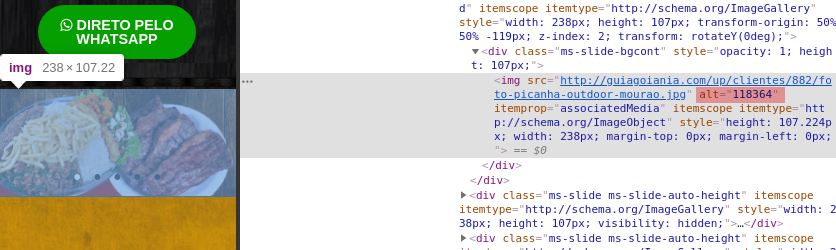
\includegraphics[scale=0.4]{images/no_alt.png}
    \caption{Site mourao restaurante}
\end{figure}

\end{frame}
\begin{frame}{Conteúdo não textual - Exemplo Bom}

Princípio: Princípio Perceptível

WCAG: 1.1 - Conteúdo não textual

\begin{itemize}
	\item Nesse site podemos ver que o que está escrito no texto também está escrito no atributo \textbf{alt}, dessa forma trazendo acessibilidade para as pessoas que tem algum problema de visão e usam algum software para poder navegar no website
\end{itemize}
\begin{figure}
    \centering
    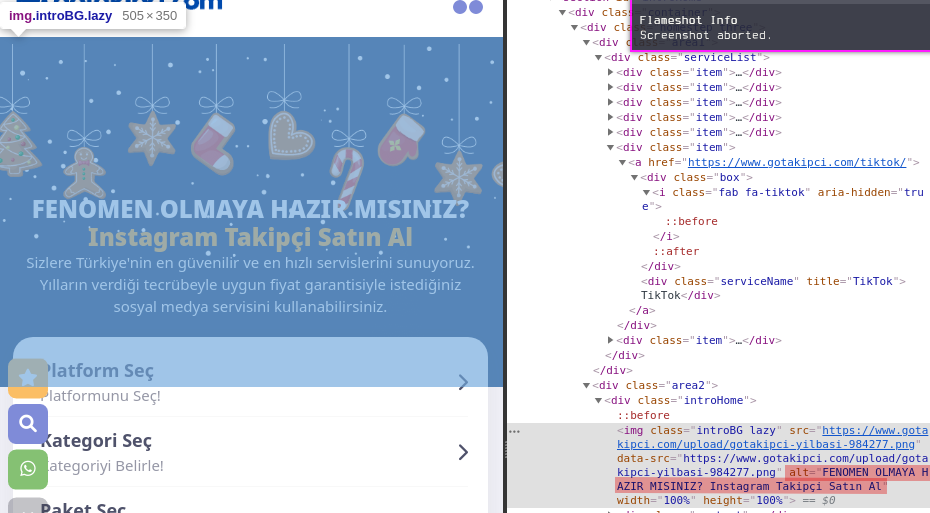
\includegraphics[scale=0.25]{images/alt.png}
    \caption{Site mourao restaurante}
\end{figure}

\end{frame}

\subsection{1.2.4 - Legendas (Ao Vivo)}

\begin{frame}{Legendas (Ao Vivo) - Exemplo Ruim}

Princípio: Princípio Perceptível

WCAG: 1.2.4 - Legendas (Ao Vivo)

\begin{itemize}
	\item A plataforma twitch não permite legenas ao vivo pela própria plataforma, e isso faz com que pessoas com deficiência auditiva não consigam acompanhar o que está acontecendo durante a transmissão
\end{itemize}
\begin{figure}
    \centering
    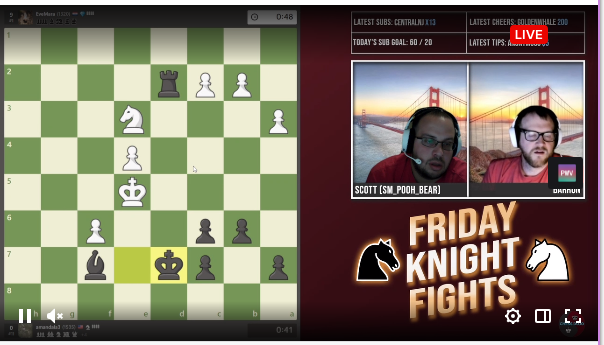
\includegraphics[scale=0.3]{images/no_subtitle.png}
    \caption{Player Twitch}
\end{figure}

\end{frame}
\begin{frame}{Legendas (Ao Vivo) - Exemplo Bom}

Princípio: Princípio Perceptível

WCAG: 1.2.4 - Legendas (Ao Vivo)

\begin{itemize}
	\item Para fazer uma transmissão ao vivo com legenda seria necessário usar um aplicativo tercerizado, um desses programas que geram legenda seria o \textbf{OBS}
\end{itemize}
\begin{figure}
    \centering
    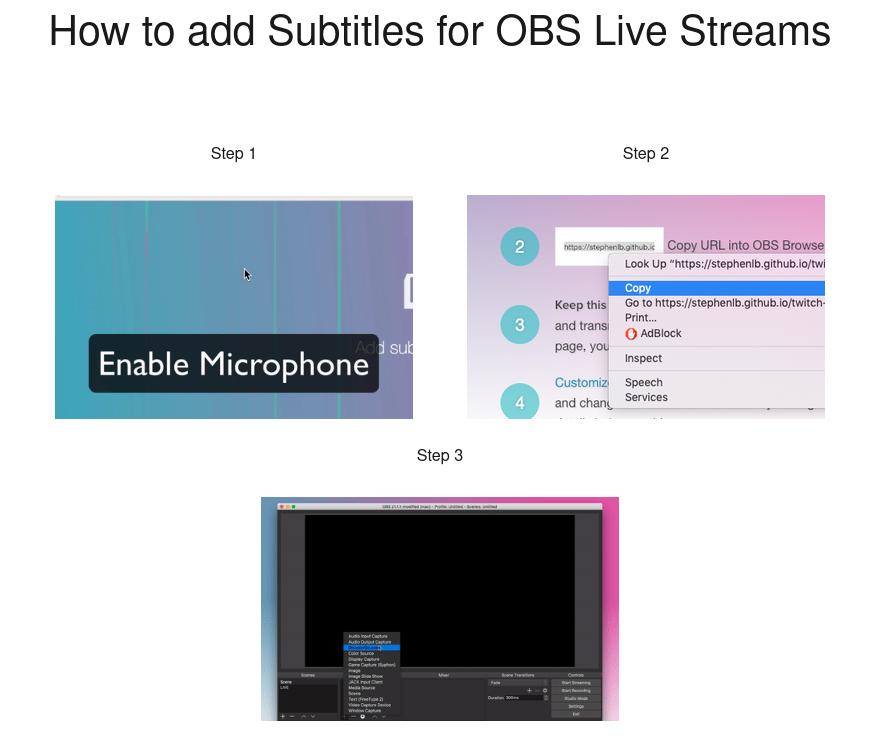
\includegraphics[scale=0.2]{images/subtitle.png}
    \caption{Legendas em uma transmissão ao vivo com o OBS}
\end{figure}
\end{frame}

\subsection{1.4.2 - Controle de Áudio}

\begin{frame}{Controle de Áudio - Exemplo Ruim}

Princípio: Princípio Perceptível

WCAG: 1.4.2 - Controle de Áudio

\begin{itemize}
	\item A página salmon of caspitrano não permite com que o usuário possa mutar ou controlar o áudio que toca no fundo
\end{itemize}
\begin{figure}
    \centering
    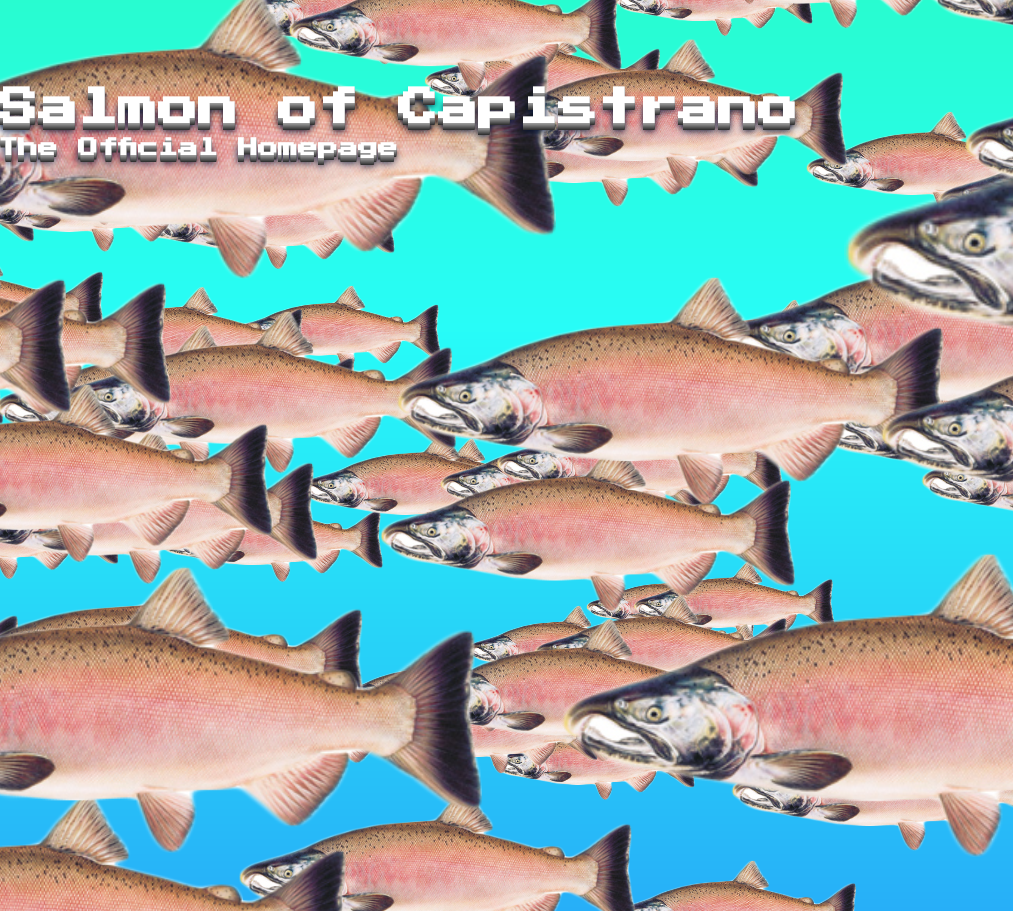
\includegraphics[scale=0.15]{images/audio.png}
    \caption{Página salmon}
\end{figure}

\end{frame}
\begin{frame}{Controle de Áudio - Exemplo Bom}

Princípio: Princípio Perceptível

WCAG: 1.4.2 - Controle de Áudio

\begin{itemize}
	\item A página cachemonet permite com que o usuário consiga desligar a música que está tocando de fundo
\end{itemize}
\begin{figure}
    \centering
    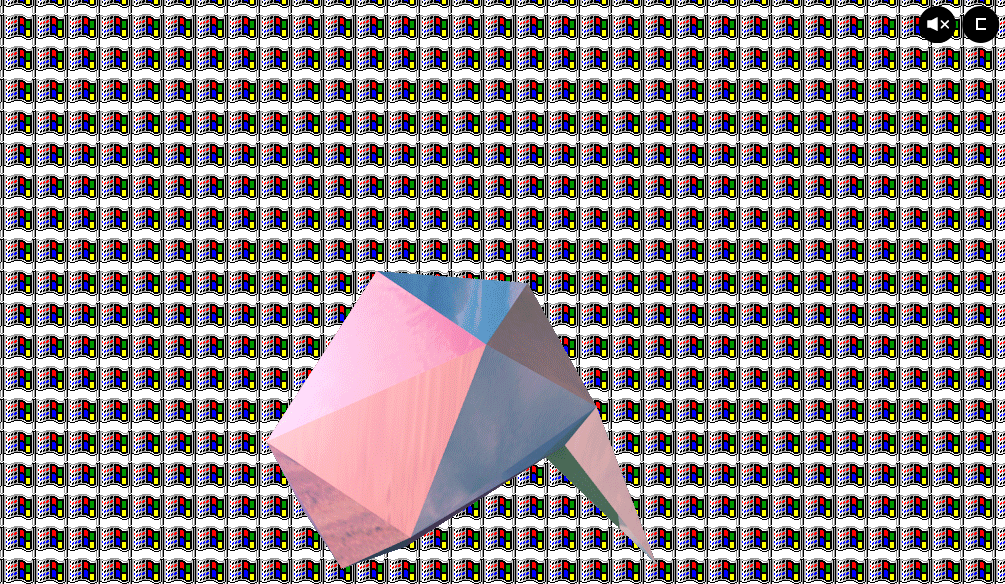
\includegraphics[scale=0.2]{images/no_audio.png}
    \caption{Página cachemonet}
\end{figure}
\end{frame}

\subsection{1.4.3 - Contraste Mínimo}

\begin{frame}{Contraste Mínimo - Exemplo Ruim}

Princípio: Princípio Perceptível

WCAG: 1.4.3 - Contraste Mínimo

\begin{itemize}
	\item Na página Randomize a sua barra de navegação contém letras com cores não muito contrastantes, o que dificulta a visão do usuário. Na esquerda é possível ver que o contraste não passaria no \textbf{WCAG AA} nem \textbf{WCAG AAA}
\end{itemize}
\begin{figure}
    \centering
    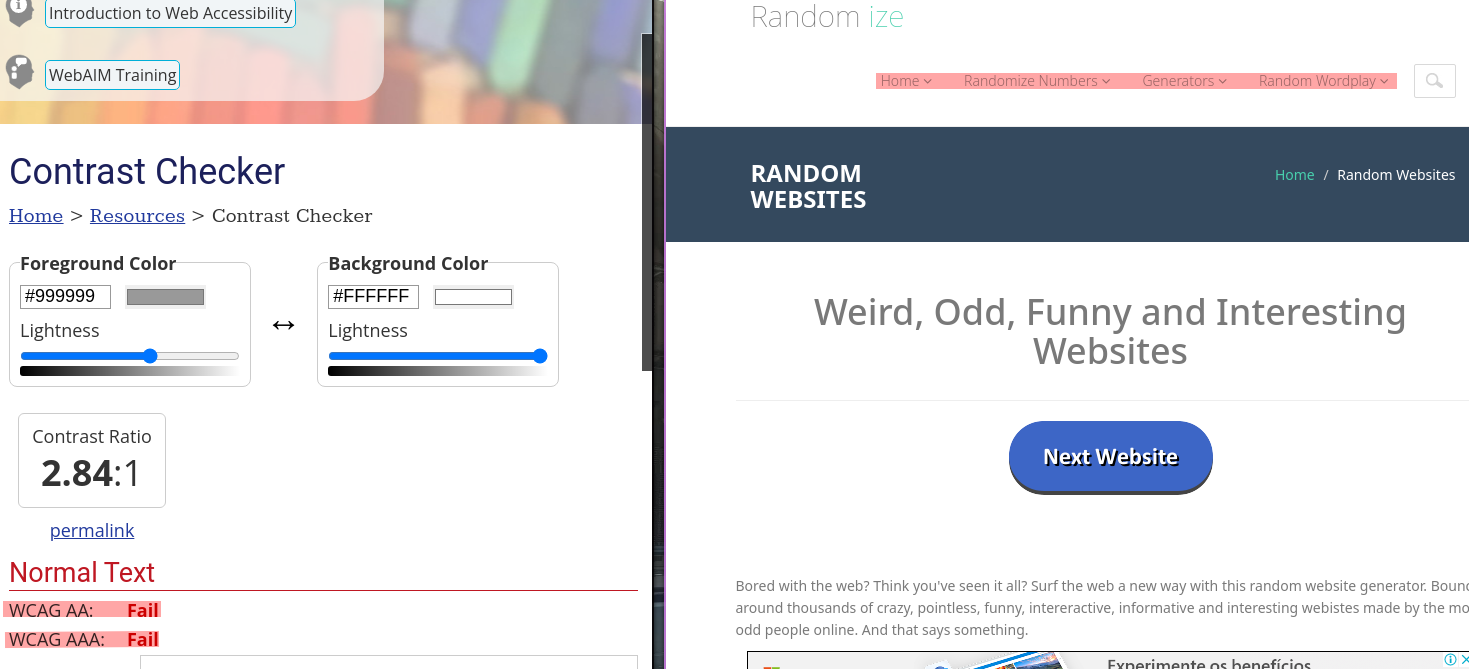
\includegraphics[scale=0.2]{images/no_contrast.png}
    \caption{Site Randomize}
\end{figure}

\end{frame}
\begin{frame}{Contraste Mínimo - Exemplo Bom}

Princípio: Princípio Perceptível

WCAG: 1.4.3 - Contraste Mínimo

\begin{itemize}
	\item Na página da documentação do software make é possível ver um contraste bom. Na esquerda é possível ver que as cores passariam no teste \textbf{WCAG AA} e no teste \textbf{WCAG AAA}
\end{itemize}
\begin{figure}
    \centering
    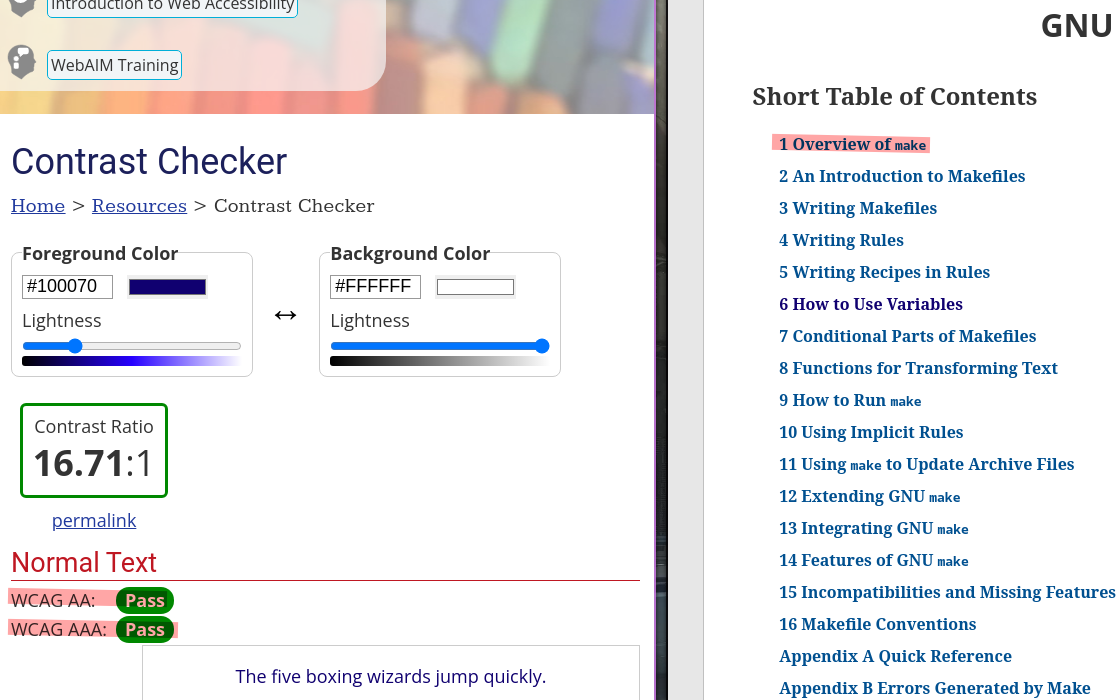
\includegraphics[scale=0.2]{images/contrast.png}
    \caption{Site GNU Make}
\end{figure}
\end{frame}

\subsection{1.4.10 - Refluxo}

\begin{frame}{Legendas (Ao Vivo) - Exemplo Ruim}

Princípio: Princípio Perceptível

WCAG: 1.4.10 - Refluxo

\begin{itemize}
	\item A página do projeto \textbf{Linux Slackware} ao dar zoom até 400\% acaba criando um scroll horizontal para que o usuário consiga ler todo o conteúdo da página
\end{itemize}
\begin{figure}
    \centering
    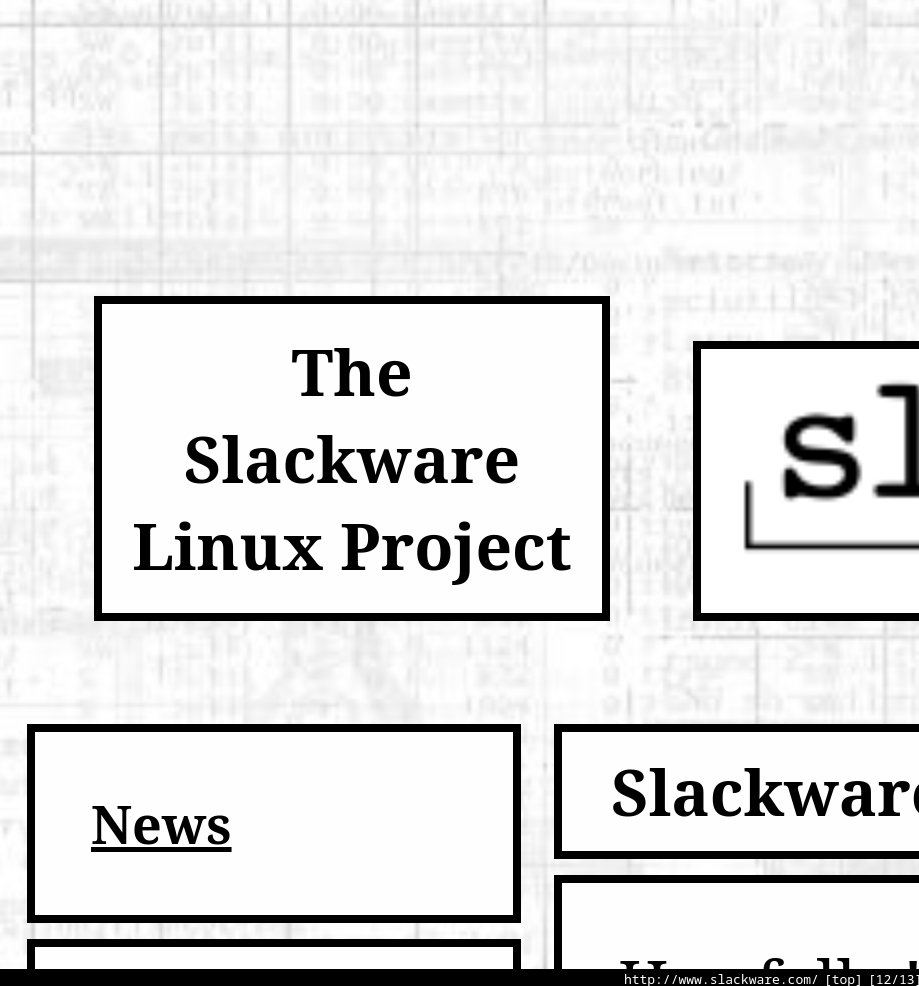
\includegraphics[scale=0.1]{images/no_refluxo.png}
    \caption{Página Projeto Linux Slackware}
\end{figure}

\end{frame}
\begin{frame}{Legendas (Ao Vivo) - Exemplo Bom}

Princípio: Princípio Perceptível

WCAG: 1.4.10 - Refluxo

\begin{itemize}
	\item A página de documentação da linguagem \textbf{Rust} permite um redimensionamento da página sem que a página crie um scroll horizontal
\end{itemize}
\begin{figure}
    \centering
    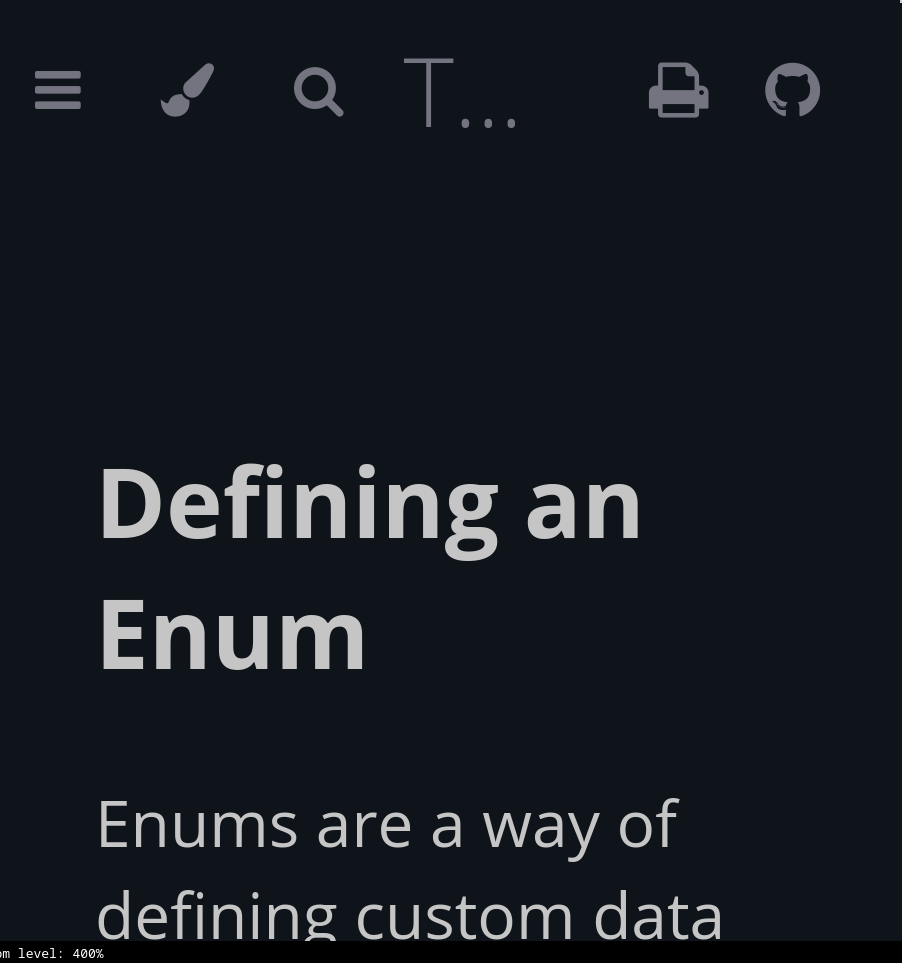
\includegraphics[scale=0.15]{images/refluxo.png}
    \caption{Documentação rust}
\end{figure}
\end{frame}

\section{Princípio Operável}
\subsection{2.1.1 - Teclado}

\begin{frame}{Teclado - Exemplo Ruim}

Princípio: Princípio Operável

WCAG: 2.1.1 - Teclado

\begin{itemize}
	\item O startpage é um website feito para pesquisa, mas na aba de imagens ao usar \textbf{tab} para navegar o usuário entra em elementos que não estão dentro da página e não é possível selecionar uma imagem usando \textbf{tab}
\end{itemize}
\begin{figure}
    \centering
    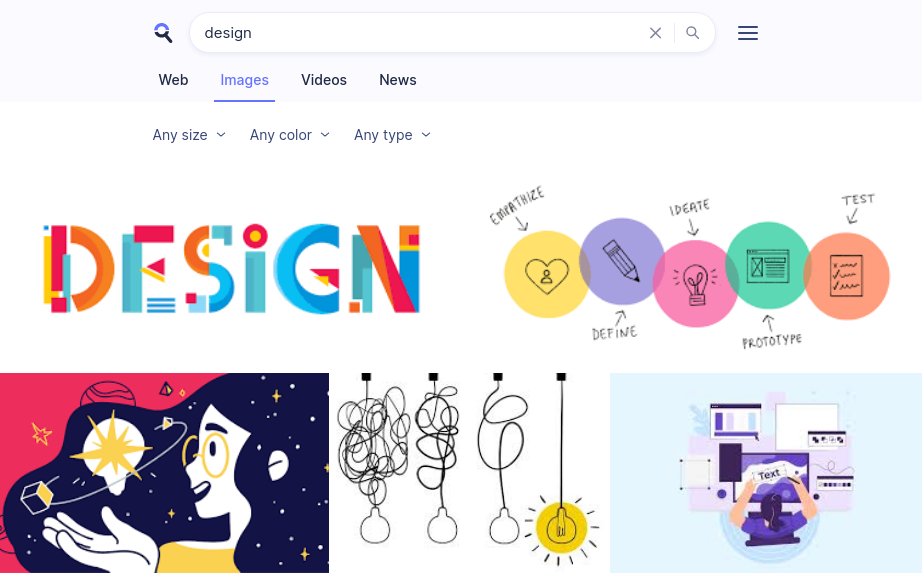
\includegraphics[scale=0.2]{images/no_keyboard.png}
    \caption{Imagens startpage}
\end{figure}

\end{frame}
\begin{frame}{Teclado - Exemplo Bom}

Princípio: Princípio Operável

WCAG: 2.1.1 - Teclado

\begin{itemize}
	\item O youtube é um bom exemplo onde podemos navegar usando a tecla \textbf{tab}para avançar  e \textbf{tab + shift} para voltar alguma opção. Ao clicar \textbf{tab}, na tela inicial por exemplo, o youtube deixa a escolha do usuário pular os botões de navegações (Imagem direita)
\end{itemize}
\begin{figure}
    \centering
    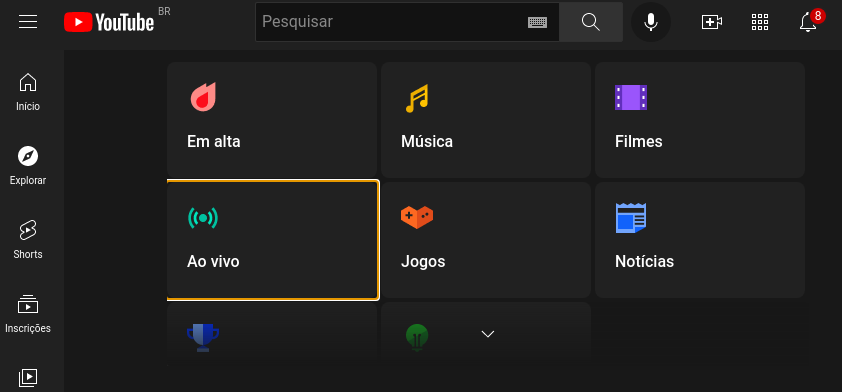
\includegraphics[scale=0.2]{images/keyboard.png}
    \caption{Selecionando uma categoria de vídeo}
\end{figure}

\end{frame}


\subsection{2.1.3 - Teclado (Sem exceção)}

\begin{frame}{Teclado (Sem exceção) - Exemplo Ruim}

Princípio: Princípio Operável

WCAG: 2.1.3 - Teclado (Sem exceção)

\begin{itemize}
	\item Usando o browser como o firefox não conseguimos acessar/selecionar as imagens no startpage
\end{itemize}
\begin{figure}
    \centering
    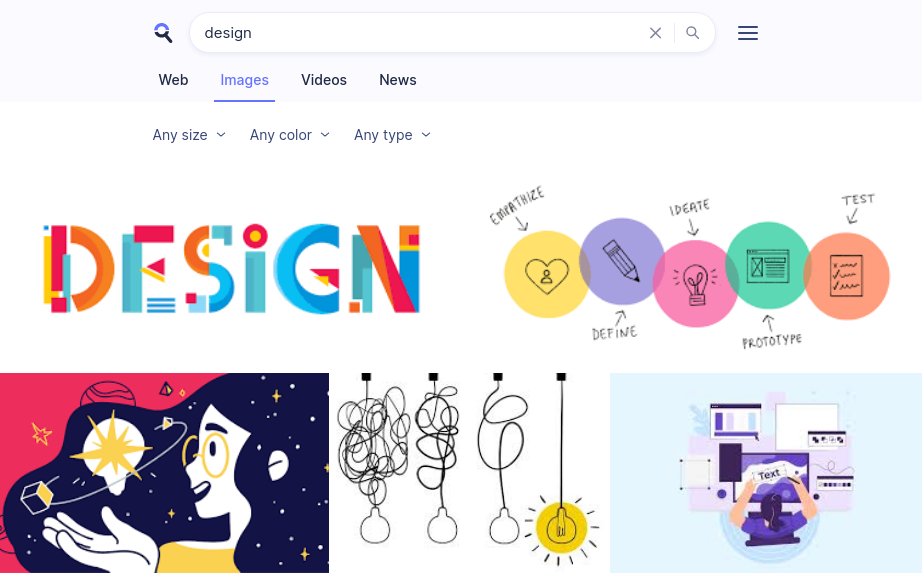
\includegraphics[scale=0.2]{images/no_keyboard.png}
    \caption{Imagens startpage}
\end{figure}

\end{frame}
\begin{frame}{Teclado (Sem exceção) - Exemplo Bom}

Princípio: Princípio Operável

WCAG: 2.1.3 - Teclado (Sem exceção)

\begin{itemize}
	\item O qutebrowser é um browser que usa atalhos baseando-se no famoso editor de texto \textbf{vim}, seu objetivo é com que o usuário consiga realizar qualquer tarefa que desejar sem precisar usar seu mouse e fazendo isso de maneira rápida e eficiente.
\end{itemize}
\begin{multicols}{2}
	\begin{figure}
	    \centering
	    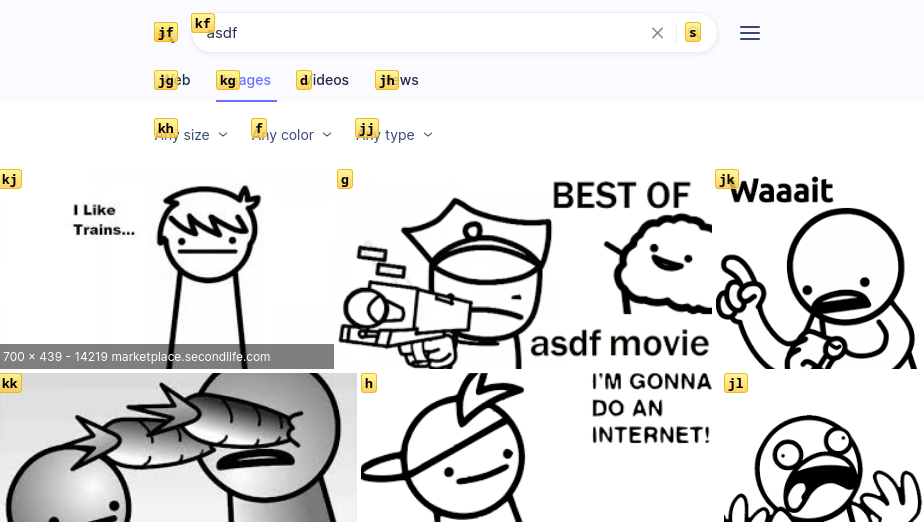
\includegraphics[scale=0.2]{images/qutebrowser.png}
	    \caption{Clicar usando o teclado}
	\end{figure}
	\begin{figure}
	    \centering
	    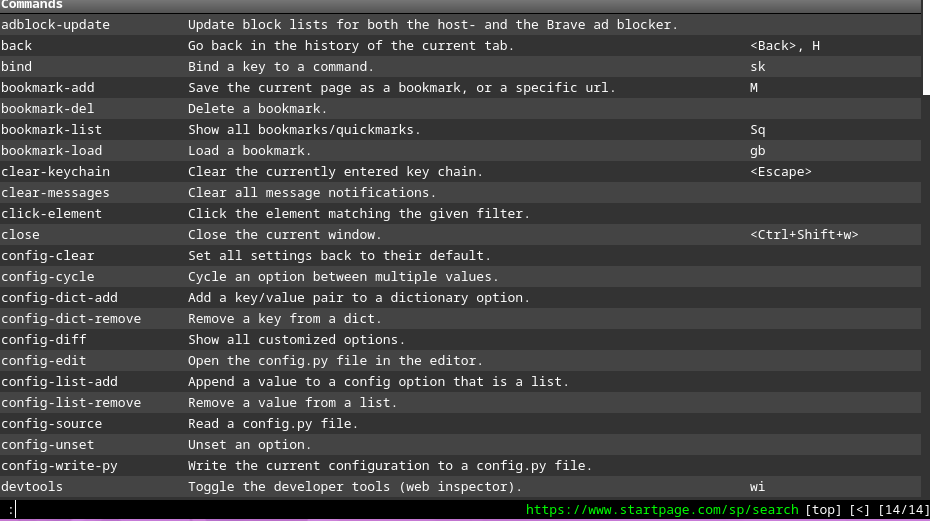
\includegraphics[scale=0.2]{images/qutebrowser1.png}
	    \caption{Usar comandos do browser}
	\end{figure}
\end{multicols}

\end{frame}

\subsection{2.4.1 - Ignorar Blocos}

\begin{frame}{Ignorar Blocos - Exemplo Ruim}

Princípio: Princípio Operável

WCAG: 2.4.1 - Ignorar Blocos

\begin{itemize}
	\item Ao usar a tecla \textbf{tab} para ser mover pela página, não conseguimos saber onde estamos e nem distinguir o que estamos selecionando com os outros objetos da página
\end{itemize}
\begin{figure}
    \centering
    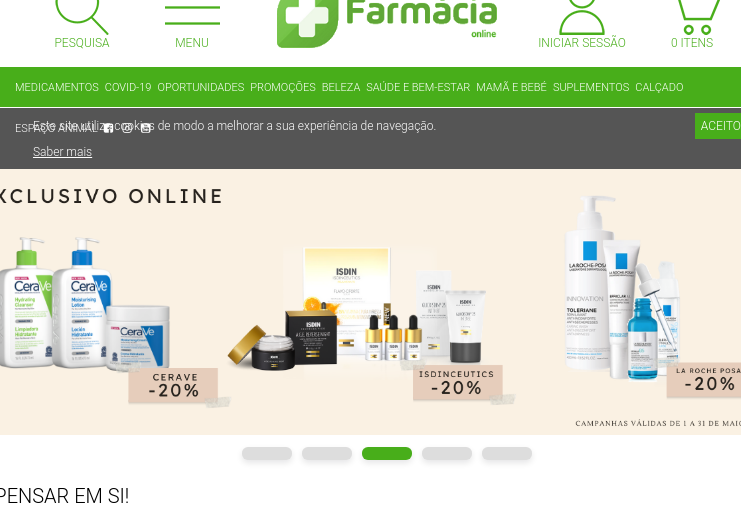
\includegraphics[scale=0.2]{images/no_ignore.png}
    \caption{Site a sua farmacia online}
\end{figure}

\end{frame}
\begin{frame}{Ignorar Blocos - Exemplo Bom}

Princípio: Princípio Operável

WCAG: 2.4.1 - Ignorar Blocos

\begin{itemize}
	\item No site do youtube temos a opção de pular a barra de navegação, dessa forma o usuário pode selecionar de maneira mais fácil os items importantes para ele
\end{itemize}
\begin{figure}
    \centering
    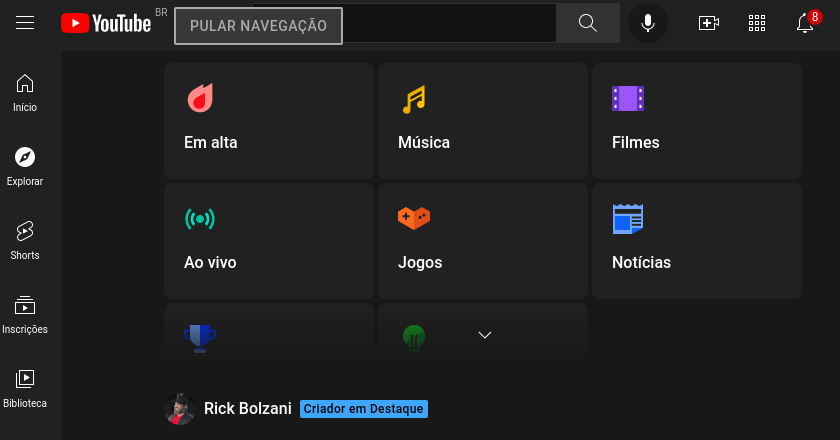
\includegraphics[scale=0.2]{images/keyboard1.png}
    \caption{Opção para pular a barra de navegação}
\end{figure}

\end{frame}

\subsection{2.4.7 - Foco Visível}

\begin{frame}{Foco Visível - Exemplo Ruim}

Princípio: Princípio Operável

WCAG: 2.4.7 - Foco Visível

\begin{itemize}
	\item Ao usar a tecla \textbf{tab} para ser mover pela página, não conseguimos saber onde estamos e nem distinguir o que estamos selecionando com os outros objetos da página
\end{itemize}
\begin{figure}
    \centering
    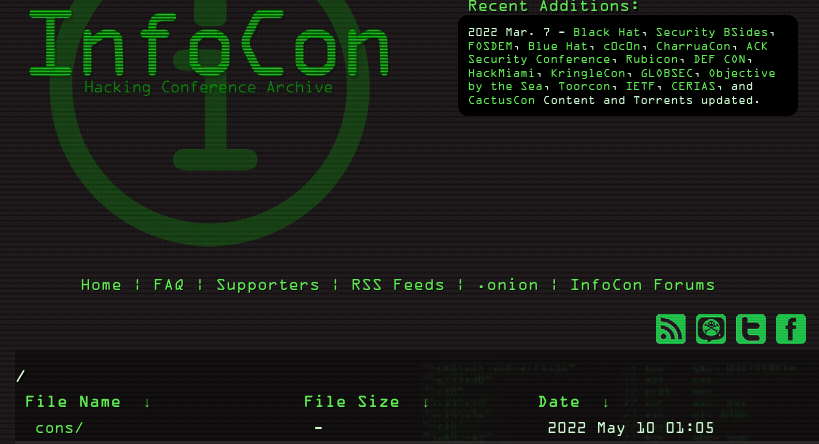
\includegraphics[scale=0.2]{images/no_focus.png}
    \caption{Infocon}
\end{figure}

\end{frame}
\begin{frame}{Foco Visível - Exemplo Bom}

Princípio: Princípio Operável

WCAG: 2.1.1 - Teclado

\begin{itemize}
	\item No site do youtube conseguimos claramente ver o que estamos selecionando
\end{itemize}
\begin{figure}
    \centering
    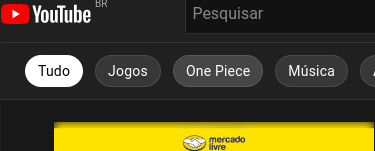
\includegraphics[scale=0.6]{images/focus.png}
    \caption{Selecionando a categoria one piece}
\end{figure}

\end{frame}

\section{Princípio Robusto}
\subsection{4.1.1 - Análise (código)}

\begin{frame}{Análise (código) - Exemplo Ruim}

Princípio: Princípio Robusto

WCAG: 4.1.1 - Análise (código)

\begin{itemize}
	\item Existem alguns erros de sintaxe na página que impedem o usuário de conseguir analisar alguns produtos, os muffins no caso da imagem abaixo:
\end{itemize}
\begin{figure}
    \centering
    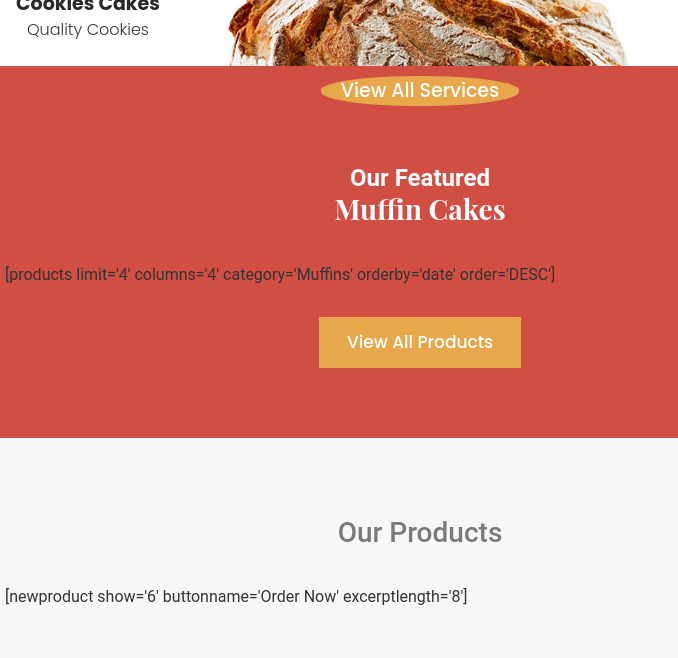
\includegraphics[scale=0.2]{images/no_code.png}
    \caption{Site maisbolosonline}
\end{figure}

\end{frame}
\begin{frame}{Análise (código) - Exemplo Bom}

Princípio: Princípio Robusto

WCAG: 4.1.1 - Análise (código)

\begin{itemize}
	\item É possível ver que o site do ifood não parece conter erros e o usuário consegue explorar tranquilamente as opções de comida
\end{itemize}
\begin{figure}
    \centering
    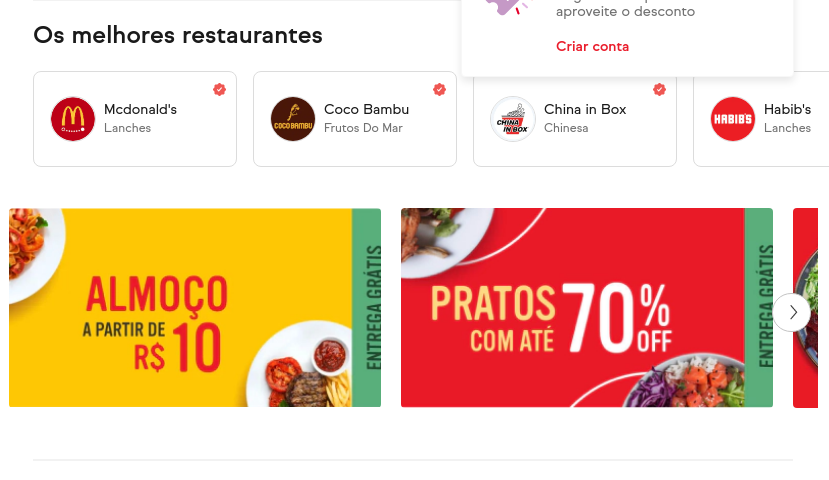
\includegraphics[scale=0.3]{images/code.png}
    \caption{Clicar usando o teclado}
\end{figure}

\end{frame}


\end{document}



